\setcounter{equation}{0} \numberwithin{equation}{section}

\section{Thoreau}
You never gain something but that you lose something.\\
		-- Thoreau
\section{Unknown}
And dropping a barbell he points to the sky\\

\begin{figure}[h]
\centering
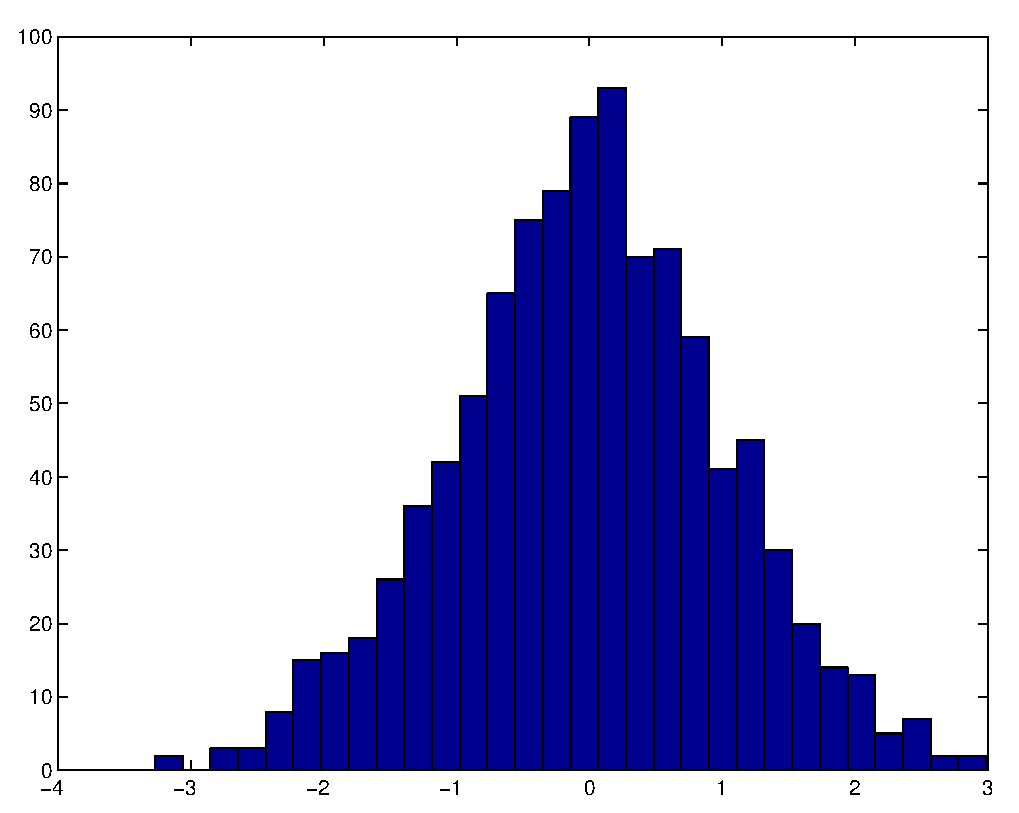
\includegraphics[width = 4.5 in ]{figure.eps}
\caption{Caption of a figure.}\label{FigureLabel}
\end{figure}

\begin{table}[h]
\centering \caption{The values of test
statistics and the corresponding critical values
at~$t_0.$~~$\alpha=0.1.$~}\label{stanford}\vskip .1in
\begin{tabular}{|c|c|c|c|c|c|c|}\hline
$t_0$ & 30 & 60 & 90 & 120 & 150 & 180 \\ \hline
Critical Value & 11.2282 & 10.5357 & 11.1108 & 11.7942 & 11.7343 & 11.7471\\ \hline
Test Statistic & 25.3182 & 24.6395 & 24.6049 & 25.6623 & 27.1320 & 29.3247\\ \hline
\end{tabular}
\end{table}

\section{Citations}

%If you use the package natbib for citations, here is the example how to cite an article.
%Many thanks to Dr. Maria Rizzo who worked this section.

To cite an article use cite, citet, or citep.

For ``in text'' citations use citet:  The original result is attributed to \citet{vn28}.
Refer to \citet{mardia70} for an example.
Refer to \cite{mardia70} for an example.

For a ``parenthetical citation'' use citep:  The computations were implemented in R \citep{R}
using bootstrap \citep{dh97,et93}.

When citing a book, it is helpful to mention where to find the result by indicating
a chapter or a page number or an equation number:  \citet[Ch.~6]{et93} discuss additional results.

Add your reference information to the file reference.bib.
Every time you edit reference.bib, run BibTeX on the dissertation.tex file so that LaTeX will know what the references are.

%If you don't want to use natbib, you should insert comment (\%) in the above part.  
%Here is the example to cite an article without using natbib package. \cite{forina1991class}


\begin{sidewaysfigure}[p!]
\centering
{bf Landscape figure}
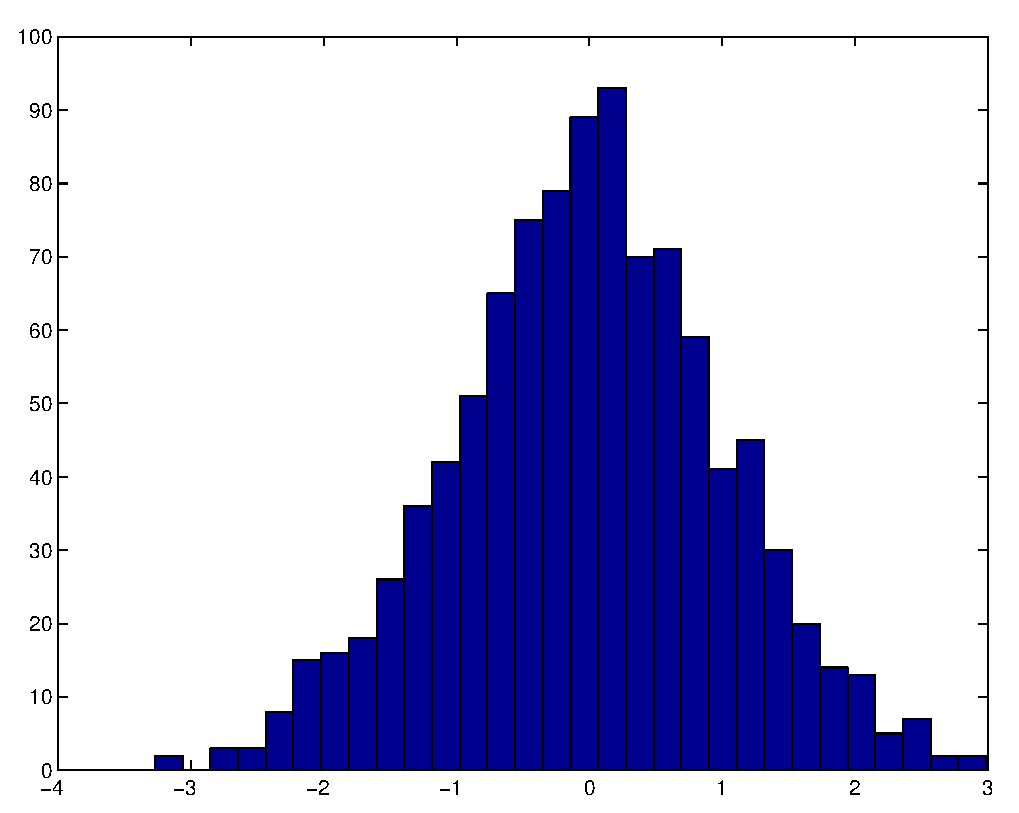
\includegraphics[width=\hsize-1in]{figure.eps}
\caption[Short label for List of Figures]{ 
Long label for under the actual figure.}
\end{sidewaysfigure}



\begin{landscape}
\thispagestyle{lscape}
\pagestyle{lscape}
  \begin{figure}
    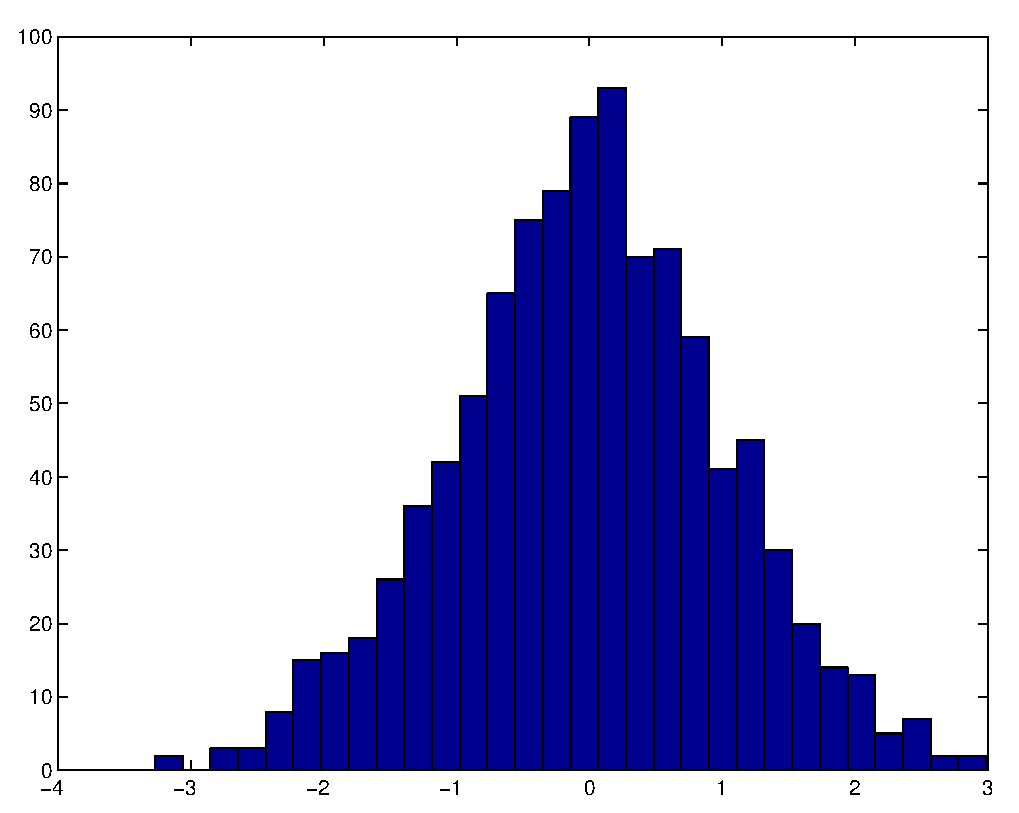
\includegraphics[width=\linewidth,height=\textheight-1in]{figure.eps}
    \caption[Short caption for List of Figures]{Long caption to appear under the figure.  Hopefully the figure is not so large that there is no room for the caption, because then the caption might move to a different page, or the text might go into the margin, and that would be bad!}
  \end{figure}
\end{landscape}
